\chapter{Einleitung}
Dieses Dokument dient der genaueren Beschreibung und Dokumentation des Entwurfs zum Visualisierungstool \gls{programname}, dessen Hauptaufgabe die Darstellung des Netzwerkverkehrs eines \gls{profinet}-Systems ist. Des Weiteren wird der im \gls{ids} \gls{snort} eingebaute \gls{praeprozessor} \gls{sppname} und die genaue Funktionsweise der \gls{ipc} zu \gls{programname} erläutert.\newline
\newline
Das Design von \gls{programname} baut auf dem klassischen \gls{mvc} auf und erweitert diesen Entwurf zu einem \gls{mvp} mit zusätzlicher Funktionalität. Das heisst, dass der Controller aufgeteilt wurde in zwei selbständige Packages. Zum Einen das Service-Package. Dabei handelt es sich um entkoppelte, selbstlaufende Routinen, welche fast die gesamte Logik des Programms ausmachen. Sie werden einmal initialisiert und laufen dann solange \gls{programname} läuft. Zum Andern gibt es den Presenter. Dieser erfüllt seine Hauptaufgabe bei Programmstart. Er instanziiert alle nötigen Klassen für den Programmablauf. Außerdem erstellt er sämtiche nötigen Referenzen, übergibt diese, und startet jeden selbständigen Thread wie zum Beispiel die Services. Danach wird der Presenter nicht mehr gebraucht.

\begin{figure}[H]
  \centering
  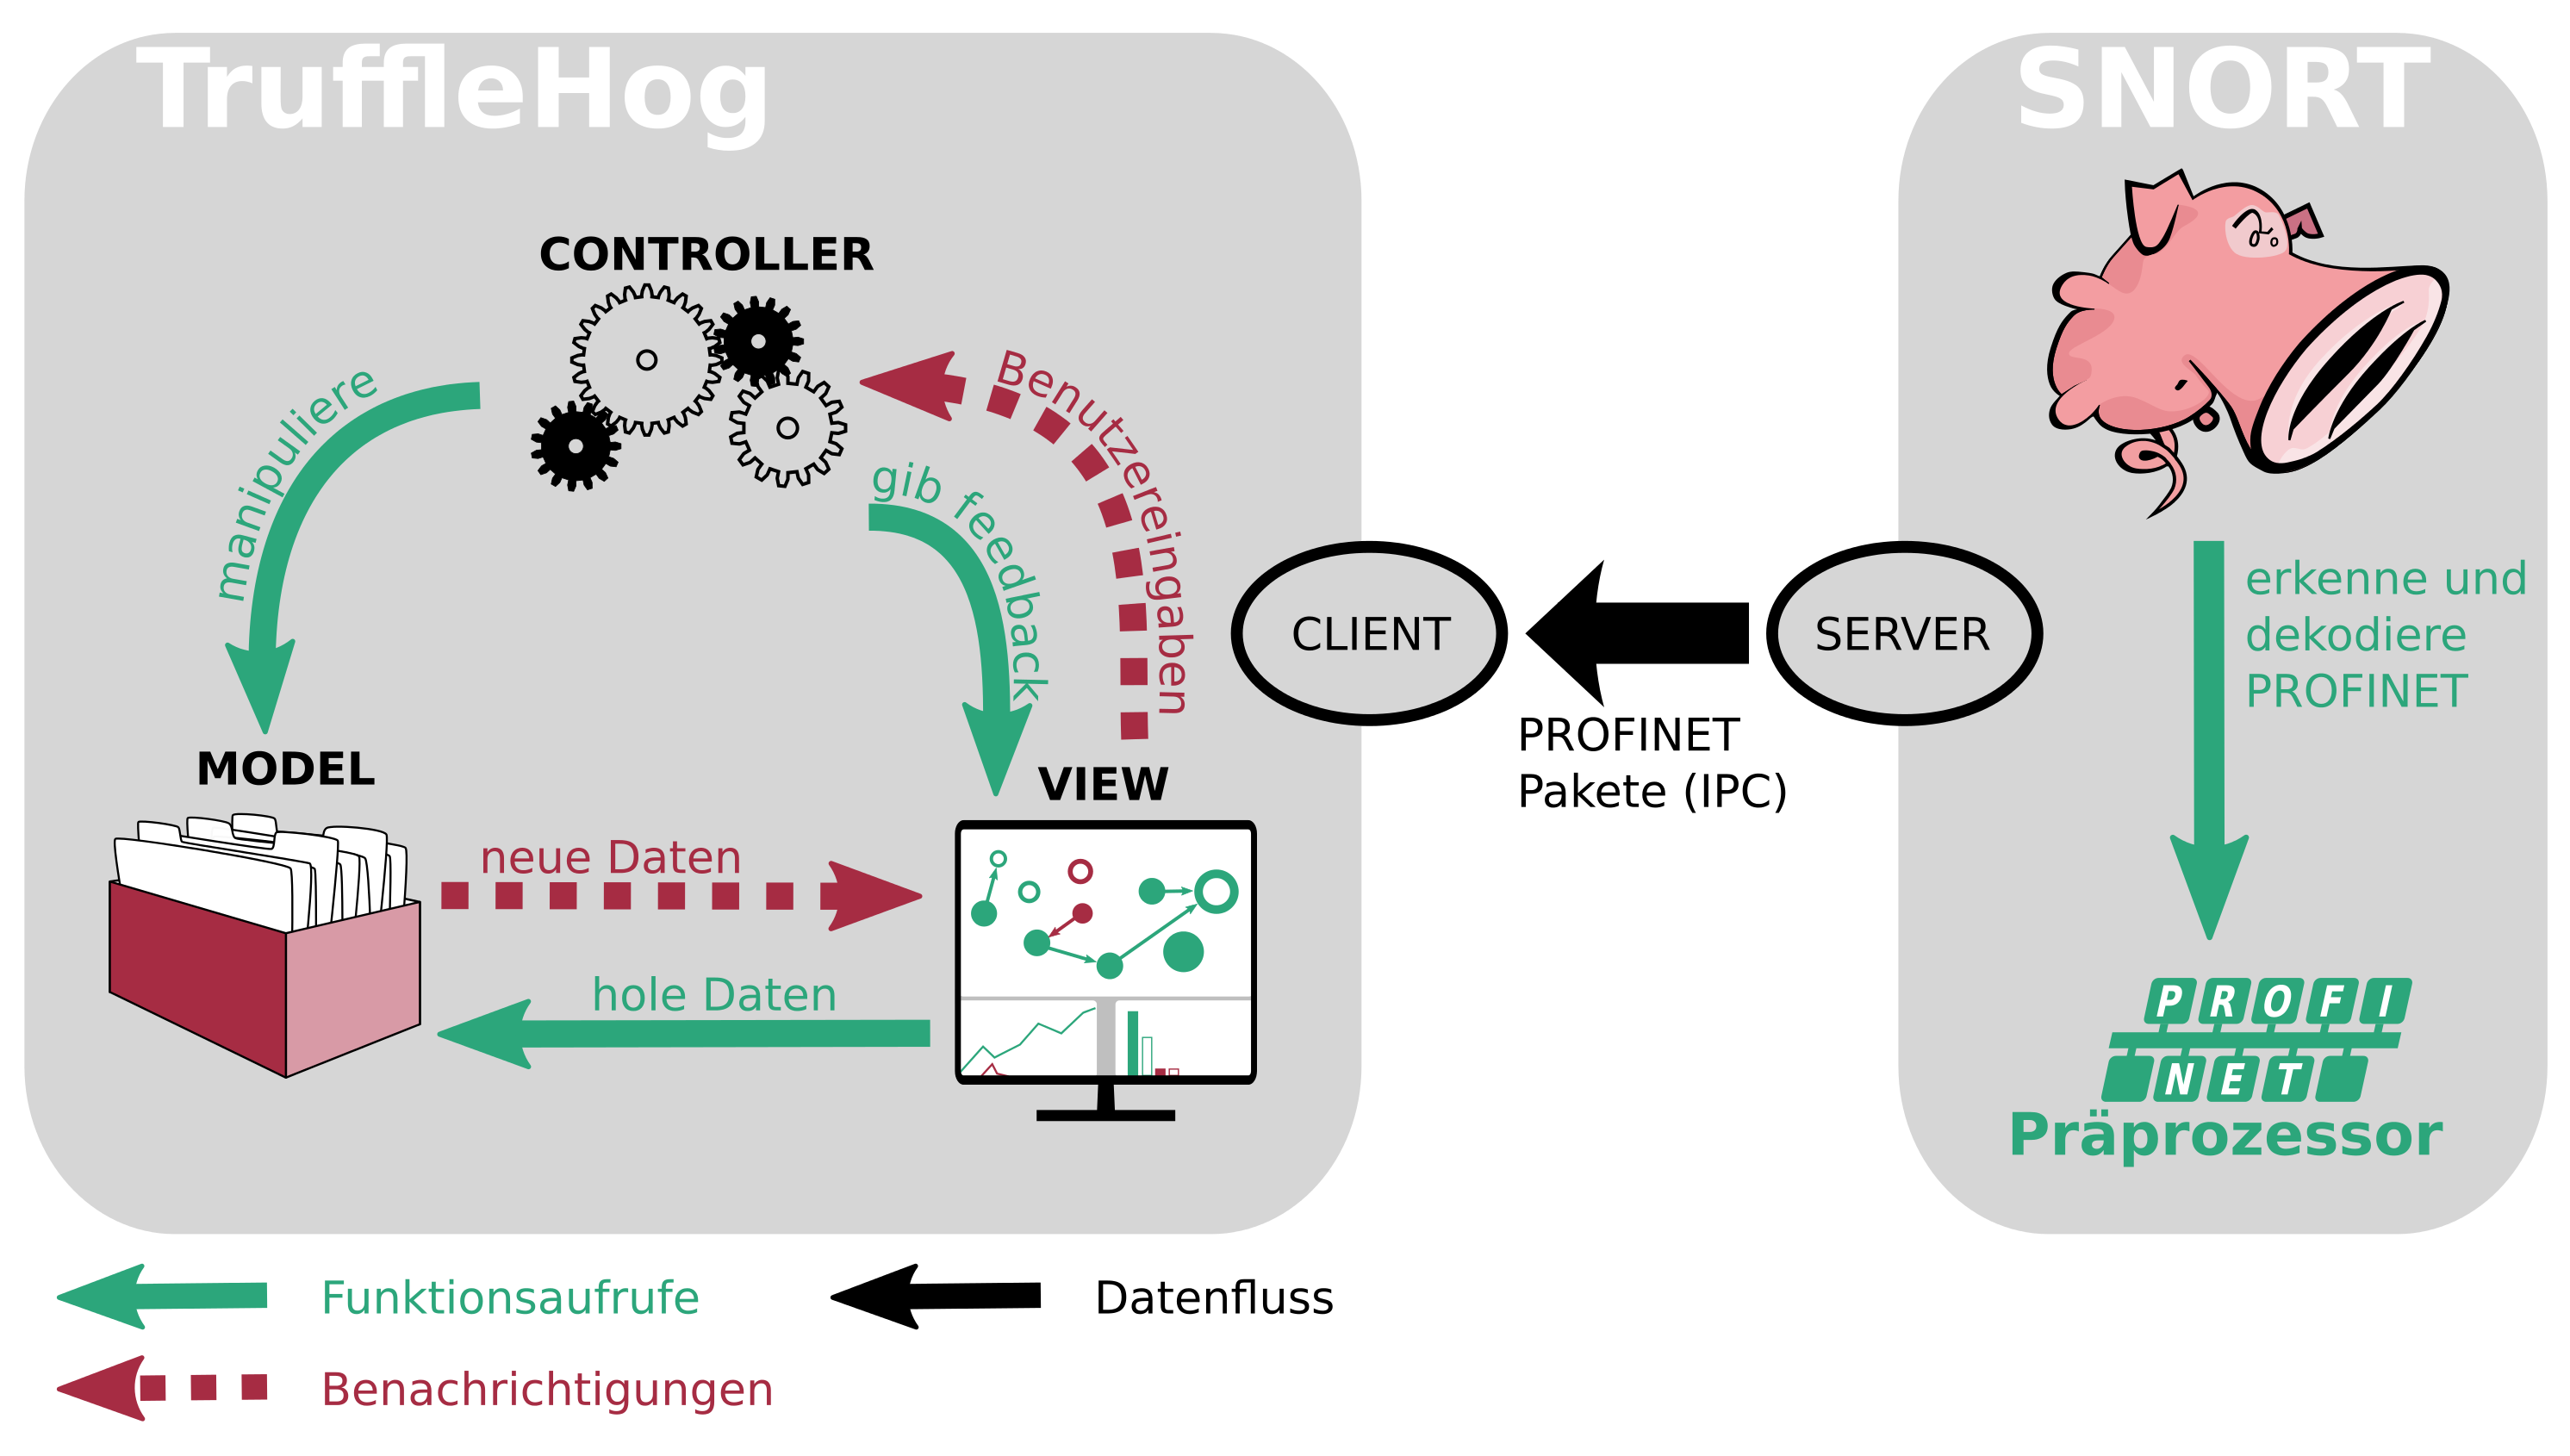
\includegraphics[width=0.8\textwidth]{../diagramimages/praesentationsmodel.png}
  \caption[\gls{mvc}]{\gls{mvc}}
  \medskip
  Grobe Struktur aus der Pflichtenheft-Präsentation
\end{figure} 